\documentclass[a4paper]{article}

\usepackage{polski}
\usepackage[utf8]{inputenc}

\usepackage[export]{adjustbox}
\usepackage{scrextend}
\usepackage{amsfonts}
\usepackage{amsmath}
\usepackage{svg}

\usepackage{geometry}
\geometry{a4paper, left=15mm, top=30mm, right=15mm, bottom=20mm}

\usepackage{gensymb}
\usepackage{graphicx} 
\usepackage{isotope}
\usepackage{array}
\usepackage{float}
\usepackage{titlesec}
\usepackage{fancyhdr}
\usepackage{multirow}

\usepackage{hyperref}
\usepackage{sectsty}
\usepackage{enumitem}
\usepackage{listings}
\usepackage[labelformat=simple]{subcaption}
\usepackage{xcolor,colortbl}
\usepackage{animate}

\sectionfont{\normalfont\huge\sectionrule{0pt}{0pt}{-6pt}{1pt}}
\subsectionfont{\normalfont\LARGE}

\pagestyle{fancy}
\fancyhf{}
\fancyhead[LE,LO]{\Large Łukasz Kwinta}
\fancyhead[RE,RO]{\Large Transfer ciepła}
\fancyfoot[CE,CO]{\Large\thepage}

\renewcommand{\footrulewidth}{1pt}
\renewcommand{\headrulewidth}{1pt}

\definecolor{Gray}{gray}{0.85}
\definecolor{LightGray}{gray}{0.95}

\newcolumntype{a}{>{\columncolor{Gray}}c}
\newcolumntype{b}{>{\columncolor{white}}c}

\title{\fontsize{30pt}{30pt}\selectfont Metoda Elementów Skończonych \\ Transfer ciepła}
\author{\fontsize{20pt}{20pt}\selectfont Łukasz Kwinta}
\date{}

\Large
\begin{document}
\maketitle
\pagebreak
\section{Wyprowadzenie sformułowania słabego}
Założenia:
\[-\frac{d}{dx}\left(k(x)\frac{du(x)}{dx}\right) = 100x \]
\[u(2) = 0\]
\[\frac{du(0)}{dx} + u(0) = 20\]
\[k(x) =
 \begin{cases}
    1  & \text{dla} x\in [0,1]\\
    2x & \text{dla} x\in (1,2]
  \end{cases}\]
  \[u: [0,2] \ni x \mapsto u(x) \in \mathbb{R}  \]

  Wyprowadzenie sformułowania słabego zaczynam od obustronnego całkowania równania 
  razem z przemnożeniem go przez funkcję testującą $\phi$:
  \[-\int_{0}^{2}(ku')'\phi dx = \int_{0}^{2}100x\phi dx\]

  Całkując lewą stronę przez części można ją uprościć:
  \[-\int_{0}^{2}(ku')'\phi dx = -\left[ku'\phi\right]_0^2 + \int_{0}^{2}ku'\phi' dx
  = -k(2)u'(2)\phi(2) + k(0)u'(0)\phi(0) + \int_{0}^{2}ku'\phi' dx = ...\]

  Korzystając z warunku Dirichleta na prawym brzegu, wiemy że $\phi(2) = 0$ co zeruje jeden człon brzegowy:
  \[... = k(0)u'(0)\phi(0) + \int_{0}^{2}ku'\phi' dx = ... \]

  Następnie korzystając z warunku Cauchego na lewym brzegu upraszczam drugi człon brzegowy:
  \[u'(0) = 20 - u(0)\]
  \[... = k(0)(20 - u(0))\phi(0) + \int_{0}^{2}ku'\phi' dx = 20k(0)\phi(0) - k(0)u(0)\phi(0) + \int_{0}^{2}ku'\phi' dx = ...\]

  Na koniec pozostało podstawić funkcję $k(x)$:
  \[... = 20\phi(0) - u(0)\phi(0) + \int_{0}^{1}u'\phi' dx + \int_{1}^{2}2xu'\phi' dx\]

  Wracając do początkowego równania przenoszę człony niezależące od $u$, na prawą stronę:
  \[20\phi(0) - u(0)\phi(0) + \int_{0}^{1}u'\phi' dx + \int_{1}^{2}2xu'\phi' dx = \int_{0}^{2}100x\phi dx\]
  \[-u(0)\phi(0) + \int_{0}^{1}u'\phi' dx + \int_{1}^{2}2xu'\phi' dx = \int_{0}^{2}100x\phi dx -20\phi(0)\]

  Niech:
  \[B(u, \phi) = -u(0)\phi(0) + \int_{0}^{1}u'\phi' dx + \int_{1}^{2}2xu'\phi' dx\]
  \[L(\phi) = \int_{0}^{2}100x\phi dx -20\phi(0)\]

  Teraz mogę zapisać sformułowanie słabe (wariacyjne). Niech
  \[ V := \left\{f \in H^1 : f(2) = 0\right\} \]
  \[\text{Szukamy:} \quad u \in V \quad \text{takiego, że:} \quad B(u, \phi) = L(\phi) \qquad \forall \phi \in V \]
  \pagebreak
  \section{Dyskretyzacja problemu}
  Jako, że $\dim V = \inf$ nie możemy rozwiązać takiego równania. Dlatego wybieramy podprzestrzeń liniową
  $V_h \subset V$
  
  Jako bazę podprzestrzeni $V_h$ bierzemy funkcje dane poniższym wzore
  \[
    e_i = 
    \begin{cases}
        \frac{x - x_{i-1}}{x_i - x_{i-1}}  & \text{dla} \quad x\in [0,1]\\
        \frac{x_{i+1} - x}{x_{i+1} - x_i}  & \text{dla} \quad x\in (1,2] \\
        0 & \text{w przeciwnym wypadku}
    \end{cases}  
  \]
  \begin{figure}[H]
    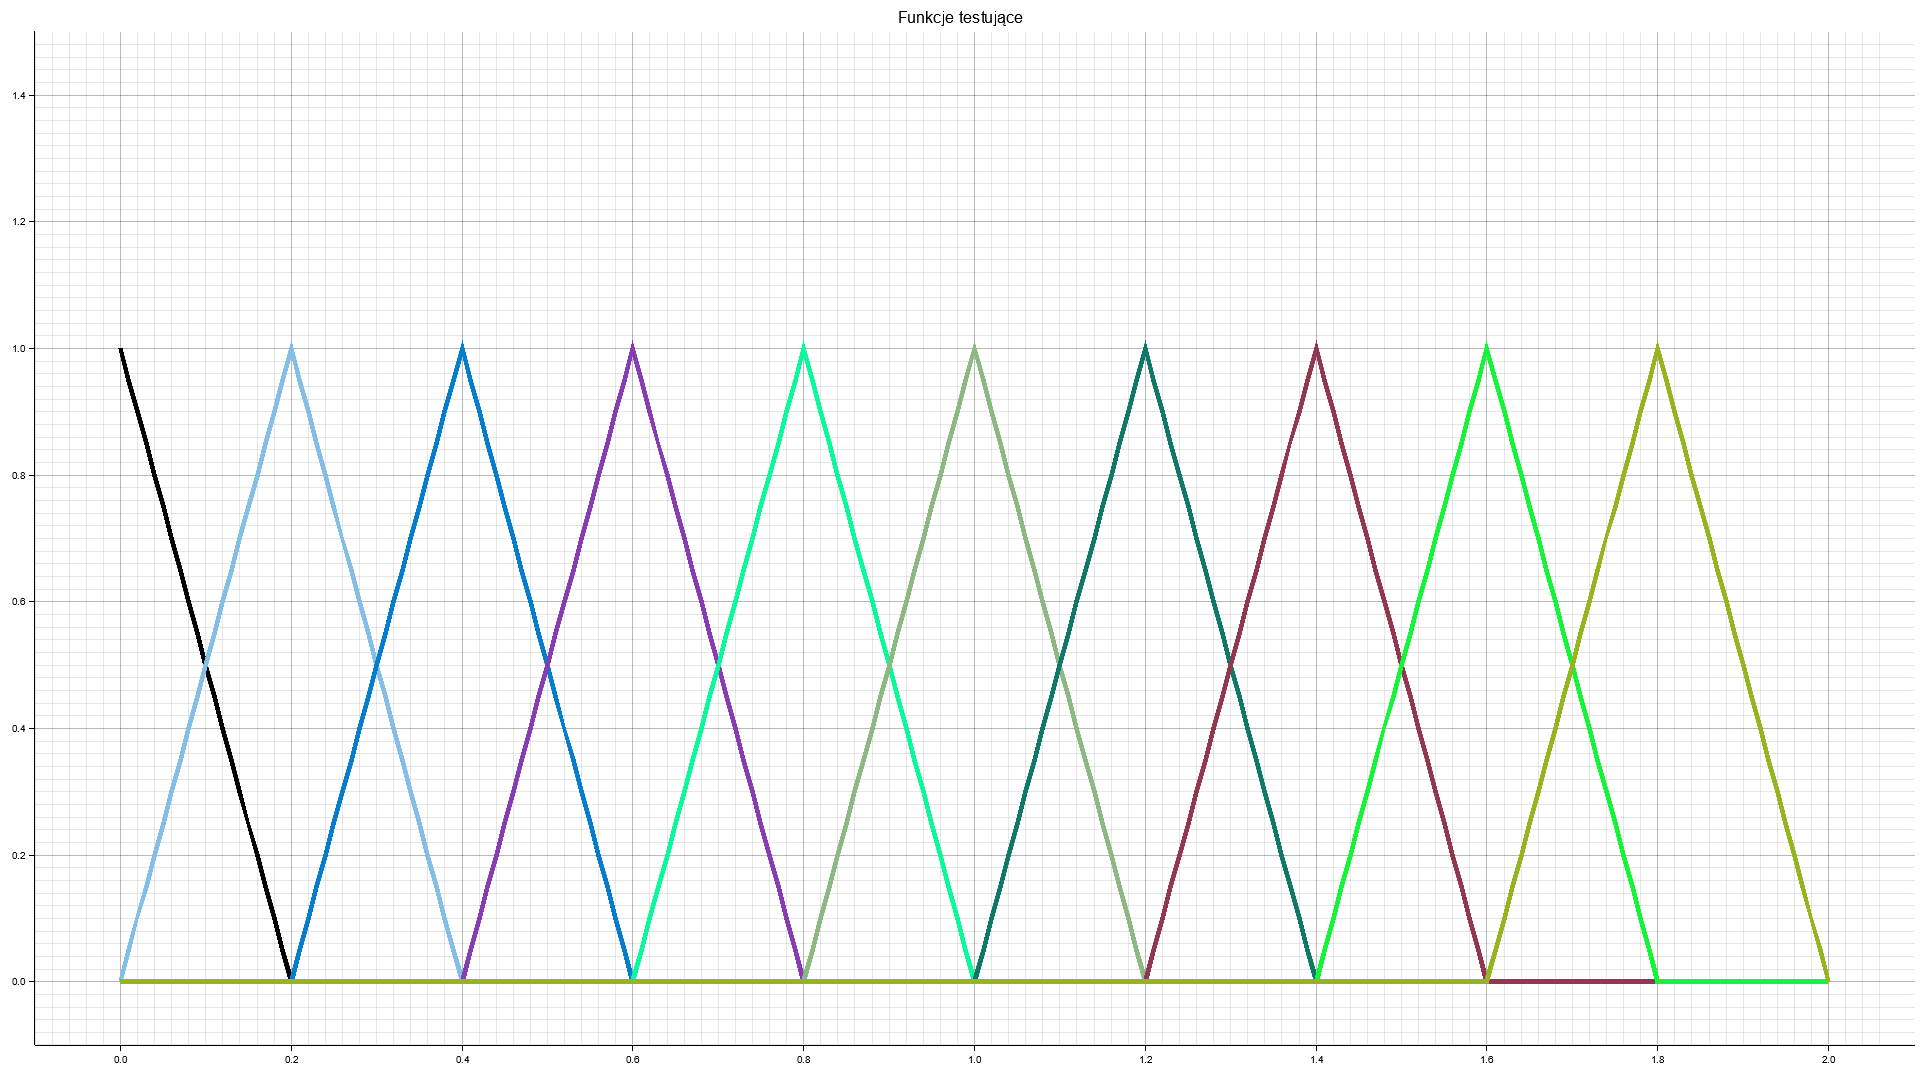
\includegraphics[width=\textwidth]{test_functions.png}
    \caption{Funkcje bazowe $e_i$ dla $N=10$}
  \end{figure}

  Jako, że na prawym brzegu mamy warunek Dirichleta, to odrzucamy funkcję $e_n$ i
  nasza podprzestrzeń będzie generowana przez następujący zbiór funkcji:
  \[V_h = span \left\{e_0, e_1, e_2, ... , e_{n-1}\right\}\]
  Sformułowanie słabe dla naszej przestrzeni dyskretnej będzie następujące:
  \[\text{Szukamy:} \quad u_h \in V_h \quad \text{takiego, że:} \quad B(u_h, \phi) = L(\phi) \qquad \forall \phi \in V_h \]
  Naszą szukaną funkcję możemy więc zapisać jako kombinację liniową funkcji z bazy podprzestrzeni:
  \[u \cong u_h = \sum_{i=0}^{n-1} e_iw_i \qquad \text{gdzie} \qquad w_i \in \mathbb{R}\]
  Sformułowanie słabe możemy teraz zapisać korzystając z funkcji z bazy:
  \[\forall_{j\in {0,1,2, ... , n-1}} : B(\sum_{i=0}^{n-1} e_iw_i, e_j) = L(e_j)\]
  Co można uprościć poprzez wyciągnięcie sumy z formy dwuliniowej:
  \[\forall_{j\in {0,1,2, ... , n-1}} : \sum_{i=0}^{n-1}w_iB(e_i, e_j) = L(e_j)\]
  Jak łatwo zauważyć, powyższe równanie jest zapisem układu równań liniowych. Można więc zapisać
  je w postaci macierzowej:\\
  \begin{center}
  $
  \left[ {\begin{array}{ccccc}
    B(e_0, e_0) & B(e_1, e_0) & B(e_2, e_0) & \cdots & B(e_{n-1}, e_0) \\
    B(e_0, e_1) & B(e_1, e_1) & B(e_2, e_1) & \cdots & B(e_{n-1}, e_1) \\
    B(e_0, e_2) & B(e_1, e_2) & B(e_2, e_2) & \cdots & B(e_{n-1}, e_2) \\
    \vdots & \vdots & \ddots & \vdots\\
    B(e_0, e_{n-2}) & B(e_1, e_{n-2}) & B(e_2, e_{n-2}) & \cdots & B(e_{n-1}, e_{n-2}) \\
    B(e_0, e_{n-1}) & B(e_1, e_{n-1}) & B(e_2, e_{n-1}) & \cdots & B(e_{n-1}, e_{n-1}) \\
  \end{array} } \right] $
  $
  \left[ {\begin{array}{c}
    w_0 \\
    w_1 \\
    w_2 \\
    \vdots \\
    w_{n-2} \\
    w_{n-1} \\
  \end{array} } \right]$ = 
  $\left[ {\begin{array}{c}
    L(e_0) \\
    L(e_1)  \\
    L(e_2)  \\
    \vdots \\
    L(e_{n-2})  \\
    L(e_{n-1})  \\
  \end{array} } \right]$
\end{center}
Rozwiązując powyższy układ równań jesteśmy w stanie wyznaczyć wagi funkcji testujących co pozwala
uzyskać przybliżone rozwiązanie problemu.
\section{Wyniki}
Po zaimplementowaniu algorytmu w języku Rust jako rozwiązanie przedstawionego problemu
uzyskałem następującą funkcję:

\begin{figure}[H]
  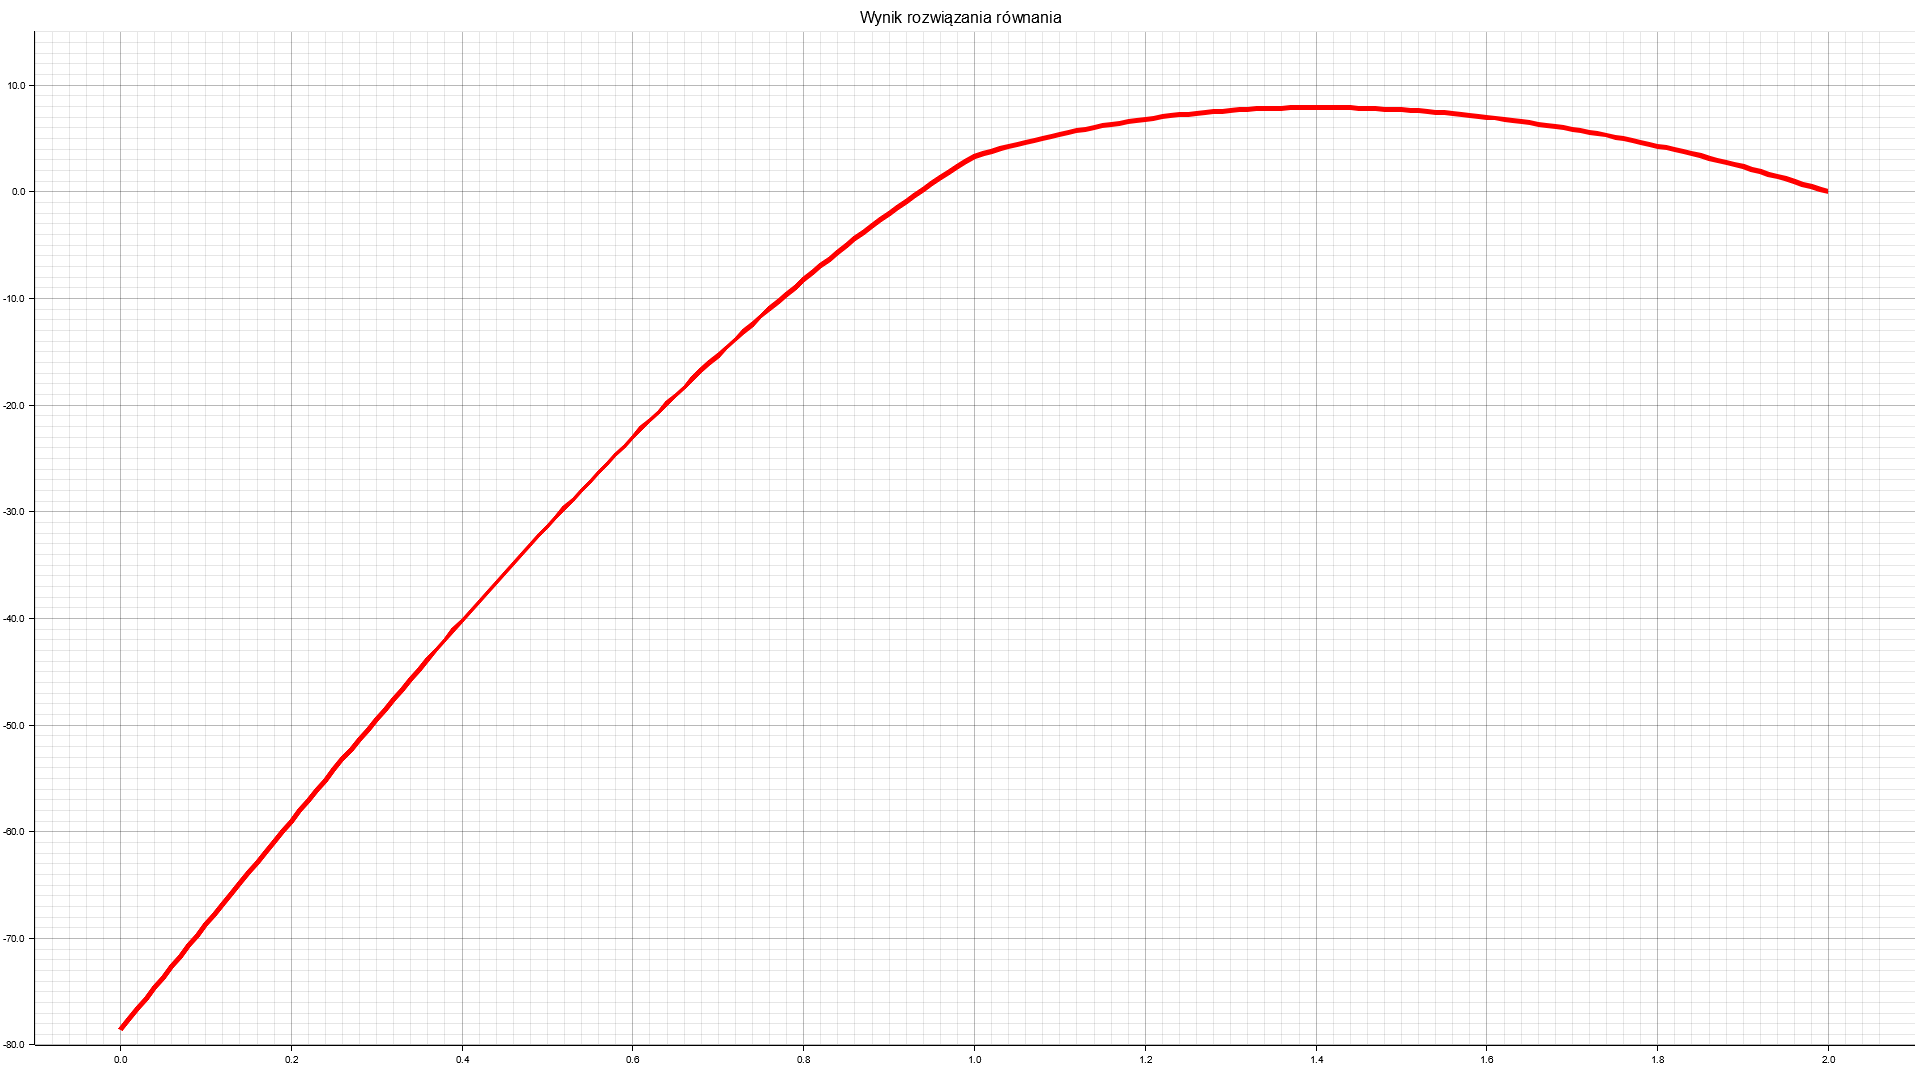
\includegraphics[width=\textwidth]{equation_result.png}
  \caption{Szukana funkcja $u(x)$ dla $N=1000$}
\end{figure}


Do obliczania całek korzystałem z kwadratury Gaussa-Legendre'a dla 3 punktów. Do rozwiązywania
układu równań liniowych urzyłem biblioteki będącej bindingie do biblioteki LAPACK.

\end{document}